\documentclass[12pt]{report}
\usepackage[spanish]{babel}
\usepackage[utf8]{inputenc}
\usepackage{amsmath}
\usepackage{amssymb}
\usepackage{amsthm}
\usepackage{graphics}
\usepackage{subfigure}
\usepackage{lipsum}
\usepackage{array}
\usepackage{multicol}
\usepackage{enumerate}
\usepackage[framemethod=TikZ]{mdframed}
\usepackage[a4paper, margin = 1.5cm]{geometry}
\usepackage{tikz}
\usepackage{pgffor}
\usepackage{ifthen}
\usepackage{enumitem}
\usepackage{hyperref}
\usepackage{bbm}
\usepackage{listings}

%Gestión de Hipervínculos

\hypersetup{
    colorlinks=true,
    linkcolor=black,
    filecolor=magenta,      
    urlcolor=cyan
}

%Gestión de Código de Programación

\definecolor{listing-background}{HTML}{F7F7F7}
\definecolor{listing-rule}{HTML}{B3B2B3}
\definecolor{listing-numbers}{HTML}{B3B2B3}
\definecolor{listing-text-color}{HTML}{000000}
\definecolor{listing-keyword}{HTML}{435489}
\definecolor{listing-keyword-2}{HTML}{1284CA} % additional keywords
\definecolor{listing-keyword-3}{HTML}{9137CB} % additional keywords
\definecolor{listing-identifier}{HTML}{435489}
\definecolor{listing-string}{HTML}{00999A}
\definecolor{listing-comment}{HTML}{8E8E8E}

\lstdefinestyle{myStyle}{
    language         = C++,
    alsolanguage     = scala,
    numbers          = left,
    xleftmargin      = 2.7em,
    framexleftmargin = 2.5em,
    backgroundcolor  = \color{gray!15},
    basicstyle       = \color{listing-text-color}\linespread{1.0}\ttfamily,
    breaklines       = true,
    frameshape       = {RYR}{Y}{Y}{RYR},
    rulecolor        = \color{black},
    tabsize          = 2,
    numberstyle      = \color{listing-numbers}\linespread{1.0}\small\ttfamily,
    aboveskip        = 1.0em,
    belowskip        = 0.1em,
    abovecaptionskip = 0em,
    belowcaptionskip = 1.0em,
    keywordstyle     = {\color{listing-keyword}\bfseries},
    keywordstyle     = {[2]\color{listing-keyword-2}\bfseries},
    keywordstyle     = {[3]\color{listing-keyword-3}\bfseries\itshape},
    sensitive        = true,
    identifierstyle  = \color{listing-identifier},
    commentstyle     = \color{listing-comment},
    stringstyle      = \color{listing-string},
    showstringspaces = false,
    label            = lst:bar,
    captionpos       = b,
}

\lstset{style = myStyle}

%Estilo del capítulo y sección

\makeatletter
\def\thickhrulefill{\leavevmode \leaders \hrule height 1ex \hfill \kern \z@}
\def\@makechapterhead#1{%
  {\parindent \z@ \raggedright
    \reset@font
    \hrule
    \vspace*{10\p@}%
    \par
    \center \LARGE \scshape \@chapapp{} \huge \thechapter
    \vspace*{10\p@}%
    \par\nobreak
    \vspace*{10\p@}%
    \par
    \vspace*{1\p@}%
    \hrule
    %\vskip 40\p@
    \vspace*{60\p@}
    \Huge #1\par\nobreak
    \vskip 50\p@
  }}

\def\section#1{%
  \par\bigskip\bigskip
  \hrule\par\nobreak\noindent
  \refstepcounter{section}%
  \addcontentsline{toc}{chapter}{#1}%
  \reset@font
  { \large \scshape
    \strut\S \thesection \quad
    #1}% 
    \hrule   
  \par
  \medskip
}

%Gestión marca de agua

\usetikzlibrary{shapes.multipart}

\newcounter{it}
\newcommand*\watermarktext[1]{\begin{tabular}{c}
    \setcounter{it}{1}%
    \whiledo{\theit<100}{%
    \foreach \col in {0,...,15}{#1\ \ } \\ \\ \\
    \stepcounter{it}%
    }
    \end{tabular}
    }

\AddToHook{shipout/foreground}{
    \begin{tikzpicture}[remember picture,overlay, every text node part/.style={align=center}]
        \node[rectangle,black,rotate=30,scale=2,opacity=0.04] at (current page.center) {\watermarktext{Cristo Daniel Alvarado ESFM\quad}};
  \end{tikzpicture}
}

%En esta parte se hacen redefiniciones de algunos comandos para que resulte agradable el verlos%

\def\proof{\paragraph{Demostración:\\}}
\def\endproof{\hfill$\blacksquare$}

\def\sol{\paragraph{Solución:\\}}
\def\endsol{\hfill$\square$}

%En esta parte se definen los comandos a usar dentro del documento para enlistar%

\newtheoremstyle{largebreak}
  {}% use the default space above
  {}% use the default space below
  {\normalfont}% body font
  {}% indent (0pt)
  {\bfseries}% header font
  {}% punctuation
  {\newline}% break after header
  {}% header spec

\theoremstyle{largebreak}

\newmdtheoremenv[
    leftmargin=0em,
    rightmargin=0em,
    innertopmargin=0pt,
    innerbottommargin=5pt,
    hidealllines = true,
    roundcorner = 5pt,
    backgroundcolor = gray!60!red!30
]{exa}{Ejemplo}[section]

\newmdtheoremenv[
    leftmargin=0em,
    rightmargin=0em,
    innertopmargin=0pt,
    innerbottommargin=5pt,
    hidealllines = true,
    roundcorner = 5pt,
    backgroundcolor = gray!50!blue!30
]{obs}{Observación}[section]

\newmdtheoremenv[
    leftmargin=0em,
    rightmargin=0em,
    innertopmargin=0pt,
    innerbottommargin=5pt,
    rightline = false,
    leftline = false
]{theor}{Teorema}[section]

\newmdtheoremenv[
    leftmargin=0em,
    rightmargin=0em,
    innertopmargin=0pt,
    innerbottommargin=5pt,
    rightline = false,
    leftline = false
]{propo}{Proposición}[section]

\newmdtheoremenv[
    leftmargin=0em,
    rightmargin=0em,
    innertopmargin=0pt,
    innerbottommargin=5pt,
    rightline = false,
    leftline = false
]{cor}{Corolario}[section]

\newmdtheoremenv[
    leftmargin=0em,
    rightmargin=0em,
    innertopmargin=0pt,
    innerbottommargin=5pt,
    rightline = false,
    leftline = false
]{lema}{Lema}[section]

\newmdtheoremenv[
    leftmargin=0em,
    rightmargin=0em,
    innertopmargin=0pt,
    innerbottommargin=5pt,
    roundcorner=5pt,
    backgroundcolor = gray!30,
    hidealllines = true
]{mydef}{Definición}[section]

\newmdtheoremenv[
    leftmargin=0em,
    rightmargin=0em,
    innertopmargin=0pt,
    innerbottommargin=5pt,
    roundcorner=5pt
]{excer}{Ejercicio}[section]

%En esta parte se colocan comandos que definen la forma en la que se van a escribir ciertas funciones%

\newcommand\abs[1]{\ensuremath{\left|#1\right|}}
\newcommand\divides{\ensuremath{\bigm|}}
\newcommand\cf[3]{\ensuremath{#1:#2\rightarrow#3}}
\newcommand\contradiction{\ensuremath{\#_c}}
\newcommand\natint[1]{\ensuremath{\left[\big|#1\big|\right]}}
\newcommand{\bbm}[1]{\ensuremath{\mathbbm{#1}}}
\newcommand{\gen}[1]{\ensuremath{\langle#1\rangle}}
\newcounter{figcount}
\setcounter{figcount}{1}

\begin{document}
    \setlength{\parskip}{5pt} % Añade 5 puntos de espacio entre párrafos
    \setlength{\parindent}{12pt} % Pone la sangría como me gusta
    \title{Notas Curso Topología Algebraica
    
    10° Escuela Oaxaqueña de Matemáticas}
    \author{Cristo Daniel Alvarado}
    \maketitle

    \tableofcontents %Con este comando se genera el índice general del libro%

    %\setcounter{chapter}{3} %En esta parte lo que se hace es cambiar la enumeración del capítulo%

    \newpage

    \chapter{Topología Algebraica}

    \section{El grupo fundamental}

    \begin{obs}
        De ahora en adelante $X$ y $Y$ serán espacios topológicos.
    \end{obs}

    \begin{mydef}
        Sean $X$ y $Y$ espacios. Dos funciones continuas $\cf{f,g}{X}{Y}$ son \textbf{homotópicas} si $\exists\cf{H}{X\times[0,1]}{Y}$ continua (una \textbf{homotopía}) tal que:
        \begin{equation*}
            H(x,0)=f(x)\textup{ y }H(x,1)=g(x),\quad\forall x\in X
        \end{equation*}
        Escribimos que $f\simeq g$.
    \end{mydef}

    \begin{mydef}
        Los espacios $X$ y $Y$ son \textbf{homotópicamente equivalentes} si $\exists\cf{f}{X}{Y}$ y $\cf{g}{Y}{X}$ funciones continuas (llamadas \textbf{equivalencias homotópicas}) tales que:
        \begin{equation*}
            f\circ g\eqsim\bbm{1}_X\quad\textup{y}\quad g\circ f=\bbm{1}_Y
        \end{equation*}
        a lo cual escribimos $X\simeq Y$.
    \end{mydef}

    \begin{obs}
        $\simeq$ define una relación de equivalencia en la clase de espacios topológicos.
    \end{obs}

    \begin{proof}
        Ejercicio.
    \end{proof}

    \begin{propo}
        Si $X$ es homeomorfo a $Y$, entonces $X\simeq Y$.
    \end{propo}

    \begin{mydef}
        Un espacio $X$ es \textbf{contráctil} si $X\simeq\left\{*\right\}$.
    \end{mydef}

    \begin{obs}
        Otra equivalencia es que $\cf{C_p}{X}{X}$ $x\mapsto p$ es homotópica a la identidad.
    \end{obs}

    \begin{exa}
        $\mathbb{R}^n,I=[0,1],\bbm{D}^n$ son contráctilces.
    \end{exa}

    \begin{mydef}
        Un subespacio $A$ de $X$ es \textbf{un retracto de $X$} si $\exists\cf{r}{X}{A}$ continua tal que $r\big|_A=\bbm{1}_A$. En este caso $r$ es llamada una \textbf{retracción}.
    \end{mydef}

    \begin{mydef}
        Dos funciones son homotópicas relativas a $A$ si para la función $\cf{H}{X\times I}{Y}$ es tal que:
        \begin{equation*}
            H(a,t)=a,\quad\forall a\in A\forall t\in I
        \end{equation*}
    \end{mydef}

    \begin{mydef}
        Un retracto $A$ de $X$ se llama \textbf{retracto por deformación} si $\cf{i\circ x}{X}{X}$ es homotópica a $\bbm{1}_X$ relativa a $A$.
    \end{mydef}

    \begin{exa}
        $X$ es contráctil si y sólo si $\forall p\in X$, $\left\{ p\right\}\subseteq X$ es un retracto por deformación.
    \end{exa}

    \begin{exa}
        $\bbm{S}^1\subseteq\bbm{C}\setminus 0$ es un retracto por deformación.
    \end{exa}

    \begin{exa}
        $\bbm{S}^1\lor\bbm{S}^1\subseteq\mathbb{C}\setminus\left\{p,q\right\}$ es un retracto por deformación (con $p\neq q$). En este caso, $\bbm{S}^1\lor\bbm{S}^1$ es la suma puntuada (o wedge). En este caso:
        \begin{equation*}
            \bbm{S}^1\lor\bbm{S}^1=\bbm{S}^1\sqcup\bbm{S}^1/x\sim y
        \end{equation*}
        donde $x$ está en la primer esfera y $y$ en la segunda.
    \end{exa}

    \begin{exa}
        $\underset{n-\textup{veces}}{\underbrace{\bbm{S}^1\lor\cdots\lor\bbm{S}^1}}$ la rosa de $n$-pétalos es una deformación de retracción de $\mathbb{C}\setminus\left\{p_1,...,p_n \right\}$.
    \end{exa}

    \begin{exa}
        El círculo central de la banda de Möbius es retracto por deformación de $X$.
    \end{exa}

    Surge naturalmente la siguiente pregunta:

    \begin{center}
        \textit{¿Cuándo dos espacios topológicos $X$ y $Y$ NO son topológicamente equivalentes?}
    \end{center}

    La topología algebraica nos da repuestas para este tipo de preguntas, ya que traducimos el problema a algo algebraico para luego resolverlo a partir de invariantes algebraicos.

    \section{Caminos y Homotopías: El grupo fundamental}

    \begin{mydef}
        Sea $X$ espacio topológico. Un \textbf{camino de $p$ a $q$ en $X$} (con $p,q\in X$) es una función continua $\cf{f}{[0,1]}{X}$ tal que $f(0)=p$ y $f(1)=q$.
    \end{mydef}
    
    \begin{mydef}
        Dos caminos $\cf{\gamma_0,\gamma_1}{[0,1]}{X}$ de $p\in X$ a $q\in X$ son \textbf{homotópicos} si $\exists\cf{H}{[0,1]\times[0,1]}{X}$ continua tal que:
        \begin{equation*}
            H\big|_{[0,1]\times\left\{0\right\}}=\gamma_0,H\big|_{[0,1]\times\left\{1\right\}}=\gamma_1
        \end{equation*}
        y, $H\big|_{\left\{0\right\}\times[0,1]}=p$ y $H\big|_{\left\{1\right\}\times[0,1]}=1$.
    \end{mydef}

    \begin{obs}
        En cierto sentido, la familia de caminos:
        \begin{equation*}
            \left\{\gamma_t=H\big|_{[0,1]\times\left\{t\right\}}\Big|t\in[0,1] \right\}
        \end{equation*}
        deforma al camino $\gamma_0$ en $\gamma_1$.
    \end{obs}

    \begin{propo}
        $\simeq$ es una relación de equivalencia en el conjunto de caminos en $X$ de $p$ a $q$.
    \end{propo}

    \begin{obs}
        Escribimos $[\gamma]$ para la clase de $\gamma$.
    \end{obs}
    
    \begin{lema}
        Sea $\cf{\gamma}{[0,1]}{X}$ un camino de $p$ a $q$ y $\cf{\varphi}{[0,1]}{[0,1]}$ continua. Entonces, $\gamma\simeq\gamma\circ\varphi$.
    \end{lema}

    En otras palabras, reparametrizar da caminos homotópicos. Más aún, da básicamnete el mismo recorrido a diferentes velocidades.

    \begin{mydef}[\textbf{Concatenación de caminos}]
        Sean $\gamma$ un camino de $p$ a $q$ en $X$ y $\mu$ un camino de $q$ a $r$. Definimos el camino $\cf{\gamma*\mu}{[0,1]}{X}$ de $p$ a $r$ como:
        \begin{equation*}
            \gamma*\mu(t)=\left\{
                \begin{array}{lcr}
                    \gamma(2t) & \textup{ si } & t\in[0,1/2]\\
                    \mu(2t-1) & \textup{ si } & t\in[1/2,1]\\
                \end{array}
            \right.
        \end{equation*}
    \end{mydef}

    \begin{mydef}
        Sea $p\in X$, $\cf{e_p}{[0,1]}{X}$ dado por: $e_p(t)=p$ para todo $t\in[0,1]$ es el \textbf{camino constante} de $p$ a $p$.
    \end{mydef}

    \begin{lema}
        Sean $\gamma_0\simeq \gamma_1$ caminos de $p$ a $q$ y $\mu_0\simeq\mu_1$ caminos de $q$ a $r$. Entonces: $\gamma_0*\mu_0\simeq\gamma_1*\mu_1$.
    \end{lema}

    \begin{lema}
        Sea $\gamma$ camino de $p$ a $q$, $\mu$ de $q$ a $r$ y $\tau$ de $r$ a $s$. Entonces, $\gamma*(\mu*\tau)\simeq(\gamma*\mu)*\tau$.
    \end{lema}

    \begin{lema}
        Sea $\gamma$ camino de $p$ a $q$. Entonces:
        \begin{equation*}
            \gamma*e_p\simeq\gamma\simeq e_p*\gamma
        \end{equation*}
    \end{lema}

    \begin{mydef}
        Sea $\gamma$ un camino de $p$ a $q$. El \textbf{camio inverso} $\cf{\overline{\gamma}}{[0,1]}{X}$ de $q$ a $p$ está dado por:
        \begin{equation*}
            \overline{\gamma}(t)=\gamma(1-t),\quad\forall t\in[0,1]
        \end{equation*}
    \end{mydef}

    \begin{lema}
        $\gamma*\overline{\gamma}\simeq e_p$, $\overline{\gamma}*\gamma\simeq e_q$ y $\overline{\overline{\gamma}}=\gamma$.
    \end{lema}

    \begin{mydef}
        Un camino es \textbf{cerrado/lazo} si sus extremos coinciden.
    \end{mydef}

    \begin{mydef}
        Decimos que $\gamma$ es un \textbf{lazo basado en $x_0\in X$} si $\gamma(0)=\gamma(1)=x_0$.
    \end{mydef}

    \begin{mydef}
        Sea $x_0\in X$. El \textbf{grupo fundamental de $X$ con punto base en $x_0$} es el conjunto $\pi_1(X,x_0)$ dado por:
        \begin{equation*}
            \pi_1(X,x_0)=\left\{[\gamma]\Big|\cf{\gamma}{[0,1]}{X}\textup{ es un lazo basado en }x_0\in X \right\}
        \end{equation*}
        con el producto dado por el inducido por la concatenación de caminos.
    \end{mydef}

    \begin{obs}
        $*$ es asociativa, $[e_{ x_0}]$ es el elemento neutro y $[\overline{\gamma}]$ es el inverso de $[\gamma]$.
    \end{obs}

    \begin{exa}
        $\pi_1(\mathbb{R}^n,x_0)=\left\{[e_{ x_0}] \right\}$.
    \end{exa}

    \begin{exa}
        Si $U\subseteq\mathbb{R}^n$ tiene forma de estrella relativo a $x_0\in\mathbb{R}^n$, entonces $\pi_1(X,x_0)=\gen{e}$.
    \end{exa}
    
    \begin{obs}
        Veremos que:
        \begin{enumerate}[label = \textit{(\alph*)}]
            \item $\pi_1(\bbm{S}^1,1)\cong\mathbb{Z}$.
            \item $\pi_1(\bbm{S}^n,x_0)\cong\gen{e}$ si $n\geq2$.
            \item $\pi_1(\mathbb{C}\setminus\left\{p,q\right\},x_0)\cong F_2$, el grupo libre en dos elementos.
        \end{enumerate}
    \end{obs}

    \begin{mydef}
        Si $X$ arco-conexo tal que $\pi(X,x_0)=\gen{e}$, $X$ es llamdo \textbf{simplemente conexo}.
    \end{mydef}

    \begin{lema}[\textbf{Cambio de punto base}]
        Sea $X$ espacio topológico y $\gamma$ un camino de $p$ a $q$. Definimos $\cf{\varphi_\gamma}{\pi_1(X,p)}{\pi_1(X,q)}$ dada por:
        \begin{equation*}
            [\delta]\mapsto[\gamma*\delta*\overline{\gamma}]
        \end{equation*}
        Entonces, $\varphi_\gamma$ es un homomorfismo de grupos que solo depende de la clase de homotopía de $\gamma$.
    \end{lema}

    \begin{lema}
        Se tiene que:
        \begin{equation*}
            \begin{split}
                \varphi_{[\gamma]}\circ\varphi_{[\overline{\gamma}]}&=\bbm{1}_{\pi_1(X,q)}\\
                \varphi_{[\overline{\gamma}]}\circ\varphi_{[\gamma]}=\bbm{1}_{\pi_1(X,p)}
            \end{split}
        \end{equation*}
    \end{lema}

    \begin{cor}
        $\varphi_{[\gamma]}$ es un isomorfismo de grupos.
    \end{cor}

    \begin{lema}
        Si $p,q$ están en la misma compontente arco-conexa, entonces $\pi_1(X,p)=\pi_1(X,q)$.
    \end{lema}

    \section{Funtorialidad}

    \begin{obs}
        Podemos ver al grupo fundamental como un funtor:
        \begin{equation*}
            \cf{\pi_1}{\textup{Top}_*}{\textup{Grp}}
        \end{equation*}
        tal que $(X,x)\mapsto\pi_1(X,x)$.
    \end{obs}

    \begin{propo}
        Sea $\cf{f}{X}{Y}$ una función continua y $\cf{\gamma}{[0,1]}{X}$ un camino de $p$ a $q$. Definimos $f_*(\gamma)=f\circ\gamma$.
        \begin{enumerate}[label = \textit{(\alph*)}]
            \item $f_*(\gamma)$ es un camino de $Y$ que une a $f(p)$ con $f(q)$.
            \item Si $\gamma\simeq\gamma'$ entonces $f_*(\gamma)\simeq f_*(\gamma')$.
            \item $\gamma$ es un camino de $p$ a $q$ implica que $f_*(\gamma*\mu)=$.
            \item Si $\cf{f}{X}{Y}$ y $\cf{g}{Y}{Z}$ son funciones continuas, entonces:
            \begin{equation*}
                g_*\circ f_*=g_*\circ f_*
            \end{equation*}
            \item $(\bbm{1}_X)_*=\bbm{1}_{\pi_1(X,x_0)}$.
        \end{enumerate}
    \end{propo}

    Con lo anteroir estamos diciendo que $\pi_1$ es un funtor covariante de la categoría de espacios topológicos puntuados en la categoría de grupos.

    \begin{theor}
        $\pi_1$ es un invariante de homeomorfismo, es decir si $X\cong Y$, entonces $\pi_1(X,x_0)\overset{f_0}{\cong}\pi_1(Y,f(x_0))$.
    \end{theor}

    \begin{lema}
        Sean $\cf{f,g}{X}{Y}$ y $x_0\in X$. Si $f\simeq g$ relativas a $x_0$, entonces:
        \begin{equation*}
            \cf{f_*=g_*}{\pi_1(X,x_0)}{\pi(Y,f(x_0))}
        \end{equation*}
    \end{lema}

    \begin{theor}
        Sea $\cf{f}{X}{Y}$ y $y_0=f(x_0)$. Si $f$ es una equivalencia de homotopía, entonces $\cf{f_*}{\pi_1(X,x_0)}{\pi(Y,f(x_0))}$ es un isomorfismo, es decir que $\pi_1$ es un invariante de homotopía.
    \end{theor}

    \begin{theor}
        Si $A$ es un retracto por deformación de $X$ y $x_0\in A$, entonces el mapeo inclusión $\cf{i}{A}{X}$ induce un homomorfismo:
        \begin{equation*}
            \cf{i_*}{\pi_1(A,x_0)}{\pi_1(X,x_0)}
        \end{equation*}
    \end{theor}

    \begin{theor}
        Sean $X$ y $Y$ espacios topológicos arco-conexos, $x_0\in X$ y $y_0\in Y$, entonces:
        \begin{equation*}
            \pi_1(X\times Y,(x_0,y_0))\cong\pi_1(X,x_0)\times\pi_1(Y,y_0)
        \end{equation*} 
    \end{theor}

    \begin{exa}
        $\pi_1(\bbm{S}^1\times\bbm{S}^1,(0,0))\cong\mathbb{Z}^2$.
    \end{exa}

    \begin{obs}
        En particular, si $X$ es contráctil, entonces:
        \begin{equation*}
            \pi_1(X\times Y,(x_0,y_0))\cong\pi_1(Y,y_0)
        \end{equation*}
    \end{obs}

    \section{Teorema de Van Kampen}

    \begin{propo}
        Sea $X=U\cup V$ donde $U$ y $V$ son abiertos arco-conexos y $U\cap V$ es arco conexo. Tomemos $x_0\in X$. Sean $\cf{i}{(U,x_0)}{(X,x_0)}$ y $\cf{j}{(V,x_0)}{(X,x_0)}$ los homomorfismos inducidos. Entonces, las imágenes de:
        \begin{equation*}
            \begin{split}
                &\cf{i_*}{\pi_1(U,x_0)}{\pi_1(X,x_0)}\\
                &\cf{j_*}{\pi_1(V,x_0)}{\pi_1(X,x_0)}\\
            \end{split}
        \end{equation*}
        generan el grupo $\pi_1(X,x_0)$, es decir que el homomorfismo inducido:
        \begin{equation*}
            \cf{\psi}{\pi_1(U,x_0)*\pi_1(V,x_0)}{\pi_1(X,x_0)}
        \end{equation*}
        es sobreyectivo.
    \end{propo}

    \begin{proof}
        La estrategia de la prueba consiste en dividir el dominio de un lazo con punto base $x_0$ en invervalos más pequeños tales que las imágenes de cada uno de estos esté en $U$ o $V$. En esencia, queremos escribir a $[\gamma]$ como producto de elementos en cada uno de los grupos fundamentales (no necesariamente va a ser grupo libre, por lo que el homomorfismo será solamente sobreyectivo!). 
    \end{proof}

    \begin{obs}
        Hay un teorema de forma más general que el anterior. Si $X=\bigcup_{\alpha\in A}U_\alpha$ todos los elementos de la unión abiertos arco-conexos con $x_0\in X$ en cada uno de ellos y cada una de las intersecciones $U_\alpha\cap U_\beta$ es arco conexa, entonces $\pi_1(X,x_0)$ está generado por las imágenes de $\cf{(i_\alpha)_*}{\pi_1(U_\alpha,x_0)}{\pi_1(X,x_0)}$.
    \end{obs}

    \begin{exa}
        Tomemos $X=\bbm{S}^2\subseteq\mathbb{R}^3$. Considere los puntos $p=(0,0,1)$ y $q=(0,0,-1)$. Consideremos los abiertos:
        \begin{equation*}
            \begin{split}
                U&=\bbm{S}^2\setminus\left\{ p\right\}\cong\mathbb{R}^2\\
                V&=\bbm{S}^2\setminus\left\{ q\right\}\cong\mathbb{R}^2\\
            \end{split}
        \end{equation*}
        se tiene que $U\cap V=\bbm{S}^2\setminus\left\{p,q\right\}$ es arco conexo, $U$ y $V$ son arco conexos y $\bbm{S}^2=U\cup V$, por lo que el homomorfismo:
        \begin{equation*}
            \cf{\psi}{\pi_1(U,x_0)*\pi_1(V,x_0)}{\pi_1(\bbm{S}^2,x_0)}
        \end{equation*}
        es epimorfismo, pero como $U$ y $V$ con contráctiles, se sigue que:
        \begin{equation*}
            \pi_1(U,x_0)*\pi_1(V,x_0)=\gen{e}
        \end{equation*}
        luego, $\pi_1(\bbm{S}^2,x_0)=\gen{e}$.
    \end{exa}

    \begin{excer}
        ¿Cuál es el grupo fundamental de $\pi_1(\bbm{S}^n,x_0)$ con $n\geq 3$? ¿Qué sucede si $n=1$?
    \end{excer}

    \begin{excer}
        Prueba que $\bbm{R}^2$ no es homeomorfo a $\bbm{R}^n$ si $n\neq 2$.
    \end{excer}

    \begin{proof}
        Suponga que son homeomrfos. Se tienen dos casos:
        \begin{itemize}
            \item $n=1$
            \item $n\geq3$. Considere el 
        \end{itemize}
    \end{proof}

    \begin{theor}[\textbf{Teorema de Seifert-Van Kampen}]
        Sea $X=U\cup V$ y $x_0\in U\cap V$ con $U,V$ y $U\cap V$ abiertos arco-conexos. Sean $\cf{i_1}{U}{X}$, $\cf{i_2}{V}{X}$ y $\cf{j_1}{U\cap V}{U}$ y $\cf{j_2}{U\cap V}{V}$ los mapeos inclusión. Entonces, el morfismo inducido por $i_1$ y $i_2$
        \begin{equation*}
            \cf{\psi}{\pi_1(U,x_0)*\pi_1(V,x_0)}{\pi_1(X,x_0)}
        \end{equation*}
        y más aún,
        \begin{equation*}
            \ker(\psi)=\gen{\gen{(j_1)_*[\gamma]\left((j_2)_*([\gamma])\right)^{-1}=[\gamma]\in\pi_1(U\cap V,x_0) }}
        \end{equation*}
        (subgrupo normal que contiene a lo de adentro) es decir,
        \begin{equation*}
            \pi_1(X,x_0)=\pi_1(U,x_0)*_{\pi_1(U\cap V,x_0)}\pi_1(V,x_0)
        \end{equation*}
        es el producto amalgamado respecto al grupo formado por la intersección.
    \end{theor}

    \begin{excer}
        Se tiene que $\pi_1(\bbm{S}^1\lor\bbm{S}^1,x_0)\cong F_2$ (probar cada detalle de la demostración junto con las homotopías deseadas).
    \end{excer}

    \begin{excer}
        $\pi_1\left(\bigvee_{ i=1}^n\bbm{S}^1,x_0\right)\cong F_n$.
    \end{excer}

    \section{Grupo Fundamental de una gráfica}

    Resulta que:
    \begin{itemize}
        \item Todo árbol es contráctil.
        \item Toda gráfica conexa tiene un árbol maximal.
    \end{itemize}

    \begin{mydef}
        Sea $X$ una gráfica. Un \textbf{subárbol maximal} es una subgráfica de $X$ que es un árbol y es tal que $V(T)=V(X)$.
    \end{mydef}

    \begin{theor}
        Sea $X$ una gráfica conexa y $x_0\in V(X)$. Entonces, $\pi_1(X,x_0)$ es un grupo libre.
    \end{theor}

    \begin{proof}
        Sea $T\subseteq X$ árbol maximal y sea $\left\{e_\alpha \right\}$ las aristas de $X$ que no están en $T$. Dividimos a $e_\alpha$ en tres intervalos, esto es:
        \begin{equation*}
            e_\alpha=e_\alpha'\cup e_\alpha''\cup e_\alpha'''
        \end{equation*}
        tal que $f_\alpha=e_\alpha'\cup e_\alpha'''$ es abierto en $e_\alpha$. Tomemos $G_\alpha=T\cup e_\alpha$ y 
        \begin{equation*}
            U_\alpha=T\cup e_\alpha\cup\left(\bigcup_{\substack{\beta\\\beta\neq\alpha}}f_\alpha \right)
        \end{equation*}
        es tal que $G_\alpha\subseteq U_\alpha$ con $U_\alpha$ abierto y $U_\alpha\simeq G_\alpha$. Entonces:
        \begin{equation*}
            \pi_1(G_\alpha,x_0)\cong\mathbb{Z}
        \end{equation*}
        se tiene que $U_\alpha\cap U_\beta$ es arco-conexo y que $\pi_1(U_\alpha\cap U_\beta)\cong\gen{e}$ ya que $U_\alpha\cap U_\beta\simeq T$. Por Van-Kampen (en su versión general, se ocupan que las intersecciones dobles y triples sean arco-conexas). Luego:
        \begin{equation*}
            \pi_1(X,x_0)\cong*_{\alpha}\pi_1(G_\alpha,x_0)\cong*_{\alpha}\bbm{Z}
        \end{equation*}
    \end{proof}

    \section{Espacios Cubrientes}

    \begin{mydef}
        Sea $B$ un espacio topológico. Un \textbf{espacio de recubrimiento de $B$} consiste de: un espacio topológico $E$, una función continua sobreyectiva $\cf{p}{E}{B}$ que satisface:
        \begin{itemize}
            \item $\forall x\in B$ existe un abierto con $x\in U_x$ tal que $p^{-1}(U)=\bigsqcup_{\alpha}V_\alpha$ y $\cf{p\Big|_{V_\alpha}}{V_\alpha}{U}$ es homeomorfismo, para todo $\alpha$.
        \end{itemize}
        $p$ es llamada \textbf{función cubriente} y $B$ es llamado \textbf{espacio base}.
    \end{mydef}

    \begin{propo}
        Sea $(E,p)$ un espacio de recubrimiento de $B$. Entonces:
        \begin{enumerate}
            \item La \textbf{fibra de $b\in B$}, $p^{-1}{b}\subseteq E$ tiene la topología discreta.
            \item $\cf{p}{E}{B}$ es una función abierta.
        \end{enumerate}
    \end{propo}

    \begin{exa}
        Dado un espacio $X$, $\cf{\bbm{1}_X}{X}{X}$ es una función cubriente.
    \end{exa}

    \begin{exa}
        Dado un espacio $X$, la función $\cf{p}{X\times\left\{1,...,n\right\}}{X}$ dada por:
        \begin{equation*}
            f(x,i)=x,\quad\forall x\in X
        \end{equation*}
        y para todo $i=1,...,n$, es una función cubriente. Este espacio no es arco-conexo ni conexo, por lo que no resulta muy interesante analizarlo.
    \end{exa}

    \begin{propo}
        Sea $\cf{p}{E}{B}$ una función cubriente. Si $B_0\subseteq B$ y $E_0=p^{-1}(B_0)$, entonces $\cf{p\Big|_{E_0}}{E_0}{B_0}$ es función cubriente.
    \end{propo}

    \begin{propo}
        Sean $\cf{p}{E}{B}$ y $\cf{p'}{E'}{B'}$ funciones cubrientes, entonces:
        \begin{equation*}
            \cf{p\times p'}{E\times E'}{B\times B'}
        \end{equation*}
        es función cubriente.
    \end{propo}

    \begin{exa}
        Si $\bbm{T}=\bbm{S}^1\times\bbm{S}^1$, entonces $\cf{p}{\bbm{R}}{\bbm{S}^1}$ tal que $s\mapsto e^{ 2\pi is}$, entonces $\cf{p\times p}{\bbm{R}^2}{\bbm{T}}$ es función cubriente.
    \end{exa}

    \section{Levantamientos}

    \begin{mydef}
        Sea $\cf{p}{E}{B}$ una función cubriente. Si $\cf{f}{X}{B}$ es una función continua, un \textbf{levantamiento de $f$} es una funcioń continua $\cf{\widetilde{f}}{X}{E}$ tal que:
        \begin{equation*}
            p\circ\widetilde{f}=f
        \end{equation*}
    \end{mydef}

    \begin{theor}
        Sea $\cf{p}{E}{B}$ una función cubriente.
        \begin{enumerate}
            \item Para cada camino $\cf{\gamma}{[0,1]}{B}$ que comienza en $x_0\in B$ y $\widetilde{x}_0\in p^{-1}(x_0)$, existe un único levantamiento $\cf{\gamma}{[0,1]}{E}$ que empieza en $\widetilde{x}_0$.
            \item Para cada homotopía $\cf{H}{[0,1]\times[0,1]}{B}$ de caminos que empiezan en $x_0\in B$ y cada $\widetilde{x}_0\in p^{-1}(x_0)$ existe un único levantamiento $\cf{\widetilde{H}}{[0,1]\times[0,1]}{B}$ que es una homotopía de caminos que comienzan en $\widetilde{x_0}$
        \end{enumerate}
    \end{theor}

    Si $\cf{p}{E}{B}$ es una función cubriente con $p(e_0)=b_0$, entonces la función $\cf{\phi}{\pi_1(B,b_0)}{p^{-1}(b_0)}$, $[\gamma]\mapsto\widetilde{\gamma}(1)$, está bien definida, donde $\widetilde{\gamma}$ es el único levantamiento de $\gamma$ que empieza en $e_0$.

    \begin{theor}
        Se tienen las siguientes propiedades de $\phi$:
        \begin{itemize}
            \item Si $E$ es arco-conexo, entonces $\phi$ es sobreyectiva.
            \item Si $E$ es simplemente conexo, entonces $\phi$ es inyectiva.
        \end{itemize}
    \end{theor}

    \begin{propo}
        Sea $\cf{p}{E}{B}$ función cubriente y $p(e_0)=b_0$.
        \begin{enumerate}
            \item El homomorfismo inducido $\cf{p_*}{\pi_1(E,e_0)}{\pi_1(B,b_0)}$ es inyectivo.
            \item El subgrupo imagen $p_{*}\left(\pi_1(E,e_0) \right)\leq\pi_1(B,b_0)$ consiste de las clases de homotopía de lazos en $B$ basados en $b_0$ cuyos levantamientos a $E$ empiezan en $e_0$ son lazos en $E$.
        \end{enumerate}
    \end{propo}

    \begin{propo}
        Sea $H=p_*\left(\pi_1(E,e_0)\right)$ la correspondencia $\cf{\phi}{\pi_1(B,b_0)}{p^{-1}(b_0)}$, $[\gamma]\mapsto\widetilde{\gamma}(1)$ induce una funición inyectiva
        \begin{equation*}
            \cf{\phi}{\pi_1(B,b_0)/H}{p^{-1}(b_0)}
        \end{equation*}
        es biyectiva si $E$ es conexo.

        En particular, $\abs{p^{-1}(b_0)}=[\pi_1(B,b_0):H]$ llamado \textbf{número de hojas de la cubierta}.
    \end{propo}

    \begin{theor}
        Sea $B$ arco-conexo, localmente arco-conexo
    \end{theor}

    \chapter{Ejercicios y Problemas}

    \section{Preeliminares: el grupo fundamental}

    \begin{obs}
        Durante todo el curso todas las funciones son continuas a menos que se diga explícitamente lo contrario.
    \end{obs}

    \begin{excer}
        Muestre que el homomorfismo de cambio de punto base $\beta_h$ depende sólo de la clase de homotopía de $h$.
    \end{excer}

    \begin{proof}
        Sea $X$ espacio topológico y $\beta$ un camino en $X$ con puntos inicial y final $p$ y $q$. Asumimos probado que $\cf{\beta_h}{\pi_1(X,p)}{\pi_1(X,q)}$ es homomorsifmo. Veamos que depende solo de la clase de homotopía.
        
        En efecto, sea $\cf{h'}{[0,1]}{X}$ otro camino homotópico a $h$ y considere el homomorfismo $\cf{\beta_{ h'}}{\pi_1(X,p)}{\pi_1(X,q)}$ dado por:
        \begin{equation*}
            \beta_{h'}([\gamma])=[h'*\gamma*\overline{h'}]
        \end{equation*}
        Sea $\gamma$ un camino en $X$ con punto base $p$, se tiene que como $h\simeq h'$, entonces por un lema $h*\gamma\simeq\gamma*h'$ y nuevamente por ese mismo lema
        \begin{equation*}
            h*\gamma*\overline{h}\simeq h'*\gamma*\overline{h'}
        \end{equation*}
        por ende,
        \begin{equation*}
            [h*\gamma*\overline{h}]=[h*\gamma*\overline{h}]
        \end{equation*}
        es decir que:
        \begin{equation*}
            \beta_{h}([\gamma])=\beta_{h'}([\gamma])
        \end{equation*}
        de forma inmediata se sigue que ambos homomorfismos son iguales.

        Ahora, suponga que $\beta_h$ y $\beta_{h'}$ son dos homomorfismos tales que:
        \begin{equation*}
            \beta_h=\beta_{h'}
        \end{equation*}
        probaremos que $h=h'$. En efecto, por la igualdad se tiene que:
        \begin{equation*}
            h*\gamma*\overline{h}\eqsim h'*\gamma*\overline{h'}
        \end{equation*}
        por ende,
        \begin{equation*}
            \gamma\simeq\overline{h}*h'*\gamma*\overline{h'}*h
        \end{equation*}
        para todo camino $\gamma$. Tomando clases sucede que:
        \begin{equation*}
            [\gamma]=[\overline{h}*h']*[\gamma]*[\overline{\overline{h}*h'}],\quad\forall [\gamma]\in\pi_1(X,p)
        \end{equation*}
        y, por la estructura de grupo de $\pi_1(X,p)$ debe tenerse que este mapeo $[\gamma]\mapsto[\overline{h}*h']*[\gamma]*[\overline{\overline{h}*h'}]$ es el homomorfismo trivial, lo cual implica que $[\overline{h}*h']$ está en el centralizador de $\pi_1(X,p)$.
    \end{proof}
    
    \begin{excer}
        Sea $\cf{f}{X}{Y}$ una función continua. Si $\cf{\alpha,\beta}{I}{X}$ son caminos homotópicos muestre que los caminos $f\circ\alpha$ y $f\circ\beta$ son homotópicos.
    \end{excer}

    \begin{proof}
        Suponga que $\cf{\alpha,\beta}{I}{X}$ son homotópicos, entonces existe una función $\cf{H}{I\times I}{X}$ continua tal que:
        \begin{equation*}
            H(s,0)=\alpha(s),H(s,1)=\beta(s),\quad\forall s\in I
        \end{equation*}
        y además,
        \begin{equation*}
            H(0,t)=\alpha(0)=\beta(0),H(1,t)=\alpha(1)=\beta(1),\quad\forall t\in I
        \end{equation*}
        Considere la función $\cf{G}{I\times I}{Y}$ dada por:
        \begin{equation*}
            G(s,t)=f\circ H(s,t)
        \end{equation*}
        como $f$ y $H$ son funciones continuas, entonces $G$ es continua y cumple por las condiciones anteriores que:
        \begin{equation*}
            G(s,0)=f(H(s,0))=f\circ\alpha(s),G(s,1)=f(H(s,1))=f\circ\beta(s),\quad\forall s\in I
        \end{equation*}
        y,
        \begin{equation*}
            G(0,t)=f(H(0,t))=f\circ\alpha(0)=f\circ\beta(0),G(1,t)=f(H(1,t))=f\circ\alpha(1)=f\circ\beta(1),\quad\forall t\in I
        \end{equation*}
        por lo cual, se sigue que los caminos $f\circ\alpha$ y $f\circ\beta$ son homotópicos.
    \end{proof}

    \begin{excer}
        Si $X_0$ es la componente conexa por caminos del espacio $X$ que contiene al punto base $x_0$, muestre que la inclusión $\cf{i}{X_0}{X}$ induce un isomorfismo $\cf{i_*}{\pi_1(X_0,x_0)}{\pi_1(X,x_0)}$ dado por $[\gamma]\mapsto[i\circ\gamma]$.

        Note que hay que mostrar que $i_*$ está bien definido, es un homomorfismo y es biyectivo.
    \end{excer}

    \begin{proof}
        Veamos que está bien definido. Sean $\gamma_1,\gamma_2$ caminos en $X_0$ con punto base $x_0$ tales que $\gamma_1\simeq\gamma_2$. Se tiene que por el ejercicio anterior que $i\circ\gamma_1\simeq i\circ\gamma_2$, luego $[i\circ\gamma_1]=[i\circ\gamma_2]$, es decir que $i_*([\gamma_1])=i_*([\gamma_2])$, por lo que $i_*$ está bien definido.

        Veamos ahora que es homeomorfismo. En efecto, sean $\gamma_1,\gamma_2$ caminos en $X_0$ con punto base $x_0$, se tiene que:
        \begin{equation*}
            \begin{split}
                i_*(\gamma_1*\gamma_2)&=[i\circ(\gamma_1*\gamma_2)]\\
            \end{split}
        \end{equation*}
        Afirmamos que:
        \begin{equation*}
            i\circ(\gamma_1*\gamma_2)\simeq (i\circ\gamma_1)*(i\circ\gamma_2)
        \end{equation*}
        En efecto, esto se tiene pues $i$ es el mapeo inclusión.
        
        Por lo cual,
        \begin{equation*}
            \begin{split}
                i_*(\gamma_1*\gamma_2)&=[(i\circ\gamma_1)*(i\circ\gamma_2)]\\
                &=[i\circ\gamma_1]*[i\circ\gamma_2]\\
                &=i_*([\gamma_1])*i_*([\gamma_2])\\
            \end{split}
        \end{equation*}
        así que $i_*$ es homeomorfismo.

        Veamos que es isomorfismo. Primero notemos que es monomorfismo. En efecto, si $\gamma$ es un camino tal que $i_*([\gamma])=[e_{ x_0}]$, entonces:
        \begin{equation*}
            i\circ\gamma\simeq e_{ x_0}
        \end{equation*}
        pero, notemos que $i\circ\gamma=\gamma$, por lo que $\gamma\simeq e_{ x_0}$, es decir que $[\gamma]=[e_{ x_0}]$.
        
        Ahora veamos que es epimorfismo. Si $\eta$ es un camino en $X$ con punto base $x_0$, por ser camino y al tenerse que $x_0\in X_0$ siendo $X_0$ componente arco-conexa de $X$, debe suceder que $\gamma([0,1])\subseteq X_0$, luego tomando $\cf{\gamma}{[0,1]}{X_0}$:
        \begin{equation*}
            \gamma(t)=\eta(t),\quad\forall t\in[0,1]
        \end{equation*}
        se sigue que $i_*([\gamma])=[\eta]$.
    \end{proof}

    \begin{excer}
        Muestre que no existen retracciones en los siguientes casos:
        \begin{enumerate}[label = \textit{(\alph*)}]
            \item $X=\mathbb{R}^3$ con $A$ cualquier subespacio homeomorfo a $\mathbb{S}^1$.
            \item $X=\mathbb{S}^1\times\mathbb{D}^2$ con $A$ su frontera $\mathbb{S}^1\times\mathbb{S}^1$.
            \item $X$ la banda de Möbius y $A$ su círculo frontera.
        \end{enumerate}
    \end{excer}

    \begin{proof}
        
    \end{proof}

    \begin{excer}
        Muestre que cualquier homomorfismo $\pi_1(\mathbb{S}^1)\rightarrow\pi_1(\mathbb{S}^1)$ puede ser realizado como el homomorfismo inducido $\psi_*$ de una función $\cf{\psi}{\mathbb{S}^1}{\mathbb{S}^1}$.
    \end{excer}

    \begin{proof}
        
    \end{proof}

    \begin{excer}
        Muestre que el complemento de un conjunto finito de puntos en $\mathbb{R}^n$ es simplemente conexo si $n\geq 3$.
    \end{excer}

    \begin{proof}
        Sea $n\geq 3$ y tomemos $\left\{x_1,...,x_m \right\}\subseteq\mathbb{R}^n$. Se tienen dos casos:
        \begin{enumerate}
            \item $0\notin\left\{x_1,...,x_m \right\}$. Existe una recta que pasa por 0 tal que no pasa por ninguno de este conjunto finito de puntos, digamos la ecuación de esta recta es:
            
        \end{enumerate}
    \end{proof}

    \begin{excer}
        Calcule el grupo fundamental del espacio obtenido de dos toros $\mathbb{S}^1\times\mathbb{S}^1$ identificando el círculo $\mathbb{S}^1\times\left\{x_0\right\}$ en un toro con el correspondiente círculo $\mathbb{S}^1\times\left\{x_0\right\}$ en el otro toro.
    \end{excer}

    \begin{sol}
        
    \end{sol}

    \begin{excer}
        Calcula el grupo fundamental de la botella de Klein, el plano proyectivo $\mathbb{R}P^2$ y $\mathbb{S}^3$.
    \end{excer}

    \begin{sol}
        
    \end{sol}

    \begin{excer}
        Calcula el grupo fundamental del complenento de un conjunto finito de puntos en $\mathbb{R}^2$.
    \end{excer}

    \begin{sol}
        
    \end{sol}

    \begin{excer}
        Demuestra que $\pi_1(\mathbb{R}^2-\mathbb{Q}^2)$ no es numerable.
    \end{excer}

    \begin{proof}
        
    \end{proof}

    \begin{excer}
        Sea $X$ el espacio cociente obtenido de $\mathbb{S}^2$ identificando el polo norte con el polo sur. Calcula $\pi_1(X)$.
    \end{excer}

    \begin{sol}
        
    \end{sol}

    \begin{excer}
        El \textbf{mapping torus $T_f$} de una función $\cf{f}{X}{X}$ es el cociente obtenido de $X\times I$ identificando cada punto $(x,0)$ con $(f(x),1)$. En el caso $X=\mathbb{S}^1\lor\mathbb{S}^1$ con $f$ preservando el punto base, calcule una presentación de $\pi_1(T_f)$ en términos del homomoorfismo inducido $\cf{f_*}{\pi_1(X)}{\pi_1(X)}$.
    \end{excer}

    \begin{sol}
        
    \end{sol}

    \begin{excer}
        Demuestre que el subespacio de $\mathbb{R}^3$ que es la unión de esferas de radio $\frac{1}{n}$ y centro $\left(\frac{1}{n},0,0\right)$ para $n=1,2,...,$ es simplemente conexo.
    \end{excer}

    \begin{proof}
        
    \end{proof}

    \begin{excer}
        Sea $X$ el subespacio de $\mathbb{R}^2$ que consiste de la unión de los círculos $C_n$ de radio $n$ y centro $(n,0)$ para $n=1,2,...$. Calcule $\pi_1(X)$.
    \end{excer}

    \begin{sol}
        
    \end{sol}

    \begin{excer}
        Calcula el grupo fundamental de cualquier árbol conexo.
    \end{excer}

    \begin{sol}
        Es trivial.
    \end{sol}

    \section{Grupo Fundamental: Definiciones y Primeros Ejemplos}

    \begin{excer}
        Haga lo siguiente:
        \begin{enumerate}[label = \textit{(\alph*)}]
            \item Prueba que $\mathbb{R}$ y $I$ son espacios contráctiles.
        \end{enumerate}
    \end{excer}

    \begin{excer}
        Sea $X\subseteq\bbm{R}^3$ la unión de $n$ lineas que pasan por el origen. Calcula $\pi_1(\mathbb{R}^3\setminus X)$.
    \end{excer}

    \begin{sol}
        
    \end{sol}

    \begin{excer}
        Si $m\geq 2$, entonces $\pi_1(\bbm{S}^m,p)\cong\gen{e}$.
    \end{excer}

    \begin{proof}
        Antes, recordemos que:
        \begin{equation*}
            \bbm{S}^{n-1}\setminus\left\{p\right\}\cong\bbm{R}^n
        \end{equation*}
        para todo $p\in\bbm{S}^{n-1}$ (esta es la proyección estereográfica $m$-dimensional). Ahora, sean $p,-p\in\bbm{S}^{m}$ puntos antipodales considere los abiertos $U,V\subseteq\bbm{S}^{m}$ dados por:
        \begin{equation*}
            \begin{split}
                U&=\bbm{S}^{ m}\setminus\left\{p\right\}\\
                V&=\bbm{S}^{ m}\setminus\left\{-p\right\}
            \end{split}
        \end{equation*}
        éstos cumplen que $\bbm{S}^{m}\cong$. Se tiene que $U\cap V$ es un conjunto arco conexo no vacío si $m\geq2$ ya que $\bbm{S}^{ m}\setminus\left\{p,-p\right\}$ es un conjunto arco conexo. En caso de que $m=1$ se tendría que el $U\cap V$ no es arco conexo. Si $m=0$ se tendría que $U\cap V=\emptyset$.
        
        Sea $x_0\in U\cap V$, por Seifert-Van Kampen el homomorfismo inducido por los mapeos inlusión de $U$ y $V$ en $\bbm{S}^{m}$, respectivamente:
        \begin{equation*}
            \cf{\psi}{\pi_1(U,x_0)*\pi_1(V,x_0)}{\pi_1(\bbm{S}^{m},x_0)}
        \end{equation*}
        es suprayectivo, por el recordatorio del inicio de la demostración se tiene que:
        \begin{equation*}
            \pi_1(U,x_0)=\pi_1(\bbm{S}^{ m}\setminus\left\{p\right\},x_0)\cong\pi_1(\bbm{R}^{ m+1},0)\cong\gen{e}
        \end{equation*}
        ya que $\bbm{R}^{m+1}$ es convexo (en particular tiene forma de estrella respecto a cualquier punto) de forma análoga:
        \begin{equation*}
            \pi_1(U,x_0)\cong\gen{e}
        \end{equation*}
        así que: $\pi_1(U,x_0)*\pi_1(V,x_0)=\gen{e}*\gen{e}=\gen{e}$, por ser $\psi$ suprayectiva debe suceder que $\pi(\bbm{S}^{m},x_0)\cong\gen{e}$.
    \end{proof}

    \begin{excer}
        Demuestra que $\bbm{R}^2$ no es homeomorfo a $\bbm{R}^n$ para $n\neq 2$.
    \end{excer}

    \begin{proof}
        Analicemos varios casos:
        \begin{enumerate}[label = \textit{(\arabic*)}]
            \item $n=1$: En caso de que fuesen homeomorfos bajo el homeomorfismo $\cf{f}{\bbm{R}^2}{\bbm{R}}$, se tendría que los conjuntos:
            \begin{equation*}
                \bbm{R}^2\setminus\left\{(0,0)\right\}\cong\bbm{R}\setminus\left\{f(0,0)\right\}
            \end{equation*}
            son homeomorfos, donde $\bbm{R}^2\setminus\left\{(0,0)\right\}$ tiene una componente conexa y $\bbm{R}\setminus\left\{f(0,0)\right\}$ tiene dos, cosa que no puede suceder ya que todo homeomorfismo preserva las componentes conexas\contradiction.
            \item $n>2$: Suponga que existe tal homeomorfismo, digamos $\cf{f}{\mathbb{R}^2}{\mathbb{R}^n}$, en particular los espacios
            \begin{equation*}
                \bbm{R}^2\setminus\left\{(0,0)\right\}\cong\mathbb{R}^n\setminus\left\{f(0,0)\right\}
            \end{equation*}
            son homeomorfos.

            \textbf{Afirmación}: $\bbm{S}^{m-1}$ es retracto de deformación de $\bbm{R}^m\setminus\left\{p\right\}$. En efecto, sea $p\in\bbm{R}^m$, como $\bbm{R}^m\setminus\left\{p\right\}\cong\bbm{R}^m\setminus\left\{0\right\}$, podemos asumir que $p=0$. Considere la función $\cf{r}{\bbm{R}^m\setminus\left\{0\right\}}{\bbm{S}^{m-1}}$ dada por:
            \begin{equation*}
                x\mapsto\frac{x}{\|x\|},\quad\forall x\in\bbm{R}^m\setminus\left\{0\right\}
            \end{equation*}
            claramente esta función es continua y es tal que $r|_{\bbm{S}^{ m-1}}=\bbm{1}_{\bbm{S}^{ m-1}}$. Veamos que:
            \begin{equation*}
                i\circ r\simeq\bbm{1}_{\bbm{R}^n\setminus\left\{0\right\}}
            \end{equation*}
            En efecto, considere la función continua $\cf{H}{I\times\bbm{R}^n\setminus\left\{0\right\}}{\bbm{R}^n\setminus\left\{0\right\}}$ dada por:
            \begin{equation*}
                H(x,t)=tx+(1-t)\frac{x}{\|x\|}
            \end{equation*}
            se tiene que que:
            \begin{equation*}
                H(x,0)=\frac{x}{\|x\|}=r(x)=i\circ r(x)
            \end{equation*}
            y,
            \begin{equation*}
                H(x,1)=x=\bbm{1}_{\bbm{R}^{m}\setminus\left\{0\right\}}(x)
            \end{equation*}
            por lo cual $i\circ r\simeq\bbm{1}_{\bbm{R}^m\setminus\left\{0\right\}}$. Por tanto, $\bbm{S}^{m-1}$ es retracto de deformación de $\bbm{R}^m\setminus\left\{p\right\}$, en particular:
            \begin{equation*}
                \pi_1(\bbm{S}^{m-1},q)=\pi_1(\bbm{R}^m\setminus\left\{p\right\},q)
            \end{equation*}
            para todo $q\in\bbm{S}^{ m-1}$.

            Ahora, como los espacios $\bbm{R}^2\setminus\left\{(0,0)\right\}$ y $\bbm{R}^n\setminus\left\{f(0,0)\right\}$ son homeomorfos y arco-conexos, se tiene que sus grupo fundamentales en cualquier punto deben ser isomorfos, es decir:
            \begin{equation*}
                \pi_1(\bbm{R}^2\setminus\left\{(0,0)\right\})\cong\pi_1(\bbm{R}^m\setminus\left\{f(0,0)\right\})
            \end{equation*}
            lo probado en la afirmación anterior implica que:
            \begin{equation*}
                \pi_1(\bbm{S}^1,q)\cong\pi_1(\bbm{S}^n,q)
            \end{equation*}
            donde $\pi_1(\bbm{S}^1,q)\cong\bbm{Z}$ y $\pi_1(\bbm{S}^1,q)\cong\gen{e}$\contradiction.
        \end{enumerate}
        Por tanto, de los dos incisos anteriores se sigue que $\bbm{R}^2$ no puede ser homeomorfo a $\bbm{R}^n$.
    \end{proof}

    \begin{excer}
        Calcula el grupo fundamental de la botella de Klein, el plano proyectivo $\bbm{R}P^2$ y $\bbm{S}^3$.
    \end{excer}

    \begin{sol}
        Por un ejercicio anterior se tiene que $\bbm{S}^3\cong\gen{e}$.
        
        Calculemos el grupo fundamental de $\bbm{R}P^2$. Antes, notemos que:
        \begin{equation*}
            \bbm{R}P^2\setminus\bbm{D}^2\cong X
        \end{equation*}
        donde $\bbm{D}^2$ es el 2-disco y $X$ es la banda de Möbius.
        \begin{figure}
            \begin{center}
                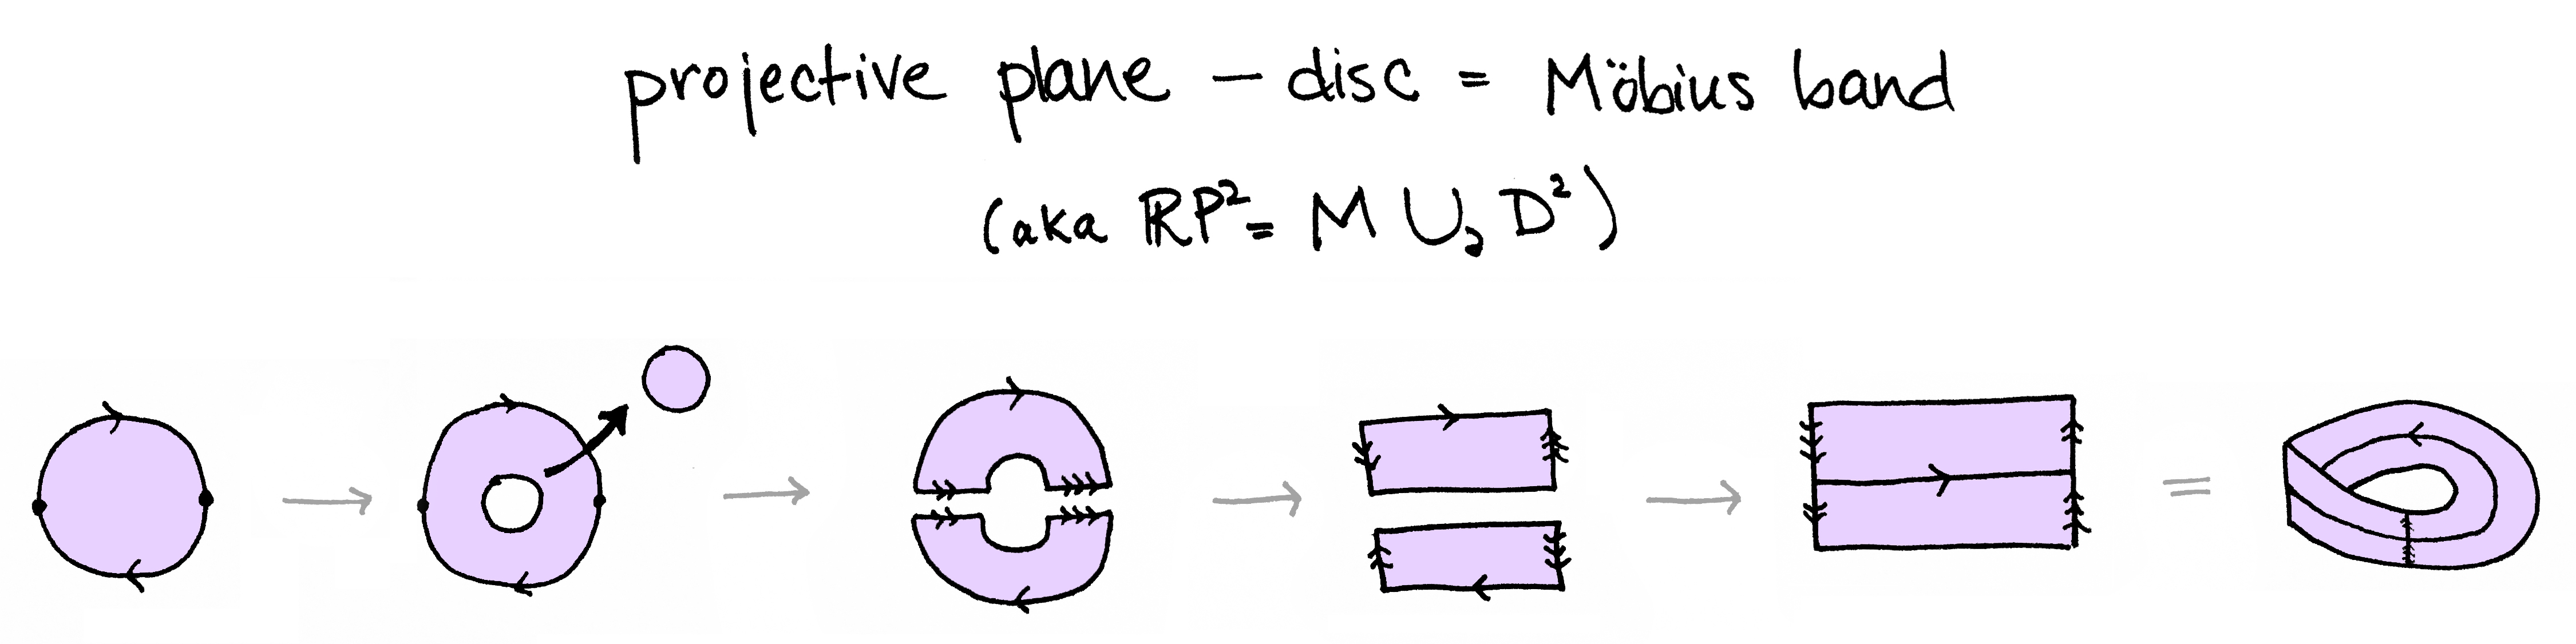
\includegraphics[scale=0.45]{constMobius.jpg}
            \end{center}
            \caption{Construcción de la banda de Möbius en el espacio $\bbm{R}P^2$.}
        \end{figure}

        Considere los abiertos $U,V\subseteq\bbm{R}P^2$ dados por: $U=\mathring{\bbm{D}^2}$ y $V=\bbm{R}P^2\setminus\widetilde{\bbm{D}^2}$, donde $\widetilde{\bbm{D}^2}\subseteq\bbm{D}^2$ es un disco de radio estrictamente menor que el radio de $\bbm{D}^2$. Se tiene que:
        \begin{equation*}
            \bbm{R}P^2=U\cup V
        \end{equation*}
        Los dos conjuntos $U$ y $V$ son arco-conexos. Además, se tiene que $U\cap V$ es arco-conexo, pues éste coincide con el conjunto:
        \begin{equation*}
            U\cap V=\mathring{\bbm{D}^2}\setminus\widetilde{\bbm{D}^2}
        \end{equation*}
        es (en términos descriptivos) un aro. Por Seifert-Van Kampen para $x_0\in U\cap V$ se tiene que:
        \begin{equation*}
            \pi_1(\bbm{R}P^2,x_0)\cong\pi_1(U,x_0)*_{\pi_1(U\cap V,x_0)}*\pi_1(V,x_0)
        \end{equation*}
        donde:
        \begin{equation*}
            \pi_1(U,x_0)=\pi_1(\mathring{\bbm{D}^2},x_0)\cong\gen{e}
        \end{equation*}
        por ser un conjunto convexo (en particular, tiene forma de estrella respecto a $x_0$), y
        \begin{equation*}
            \pi_1(V,x_0)=\pi_1(\bbm{R}P^2\setminus\widetilde{\bbm{D}^2},x_0)\cong\pi(X,y_0)
        \end{equation*}
        siendo $\pi_1(X,y_0)$ el grupo fundamental de la banda de Möbius, el cuál es $\pi_1(\bbm{S}^1,y_0)\cong\bbm{Z}$. Finalmente:
        \begin{equation*}
            \pi_1(U\cap V)\cong\bbm{Z}
        \end{equation*}
        ya que $U\cap V$ es homotópico a $\bbm{S}^1$, con grupo fundamental $\bbm{Z}$. Por ende:
        \begin{equation*}
            \pi_1(\bbm{R}P^2,x_0)\cong\gen{e}*_{\bbm{Z}}\bbm{Z}
        \end{equation*}
        Calculemos este grupo. Recordemos que:
        \begin{equation*}
            \gen{e}*\bbm{Z}/\gen{\gen{R}}
        \end{equation*}
        donde:
        \begin{equation*}
            R=\left\{(i_1)_*([\gamma])(i_2)_*([\gamma])^{-1}\Big|[\gamma]\in\pi_1(U\cap V,x_0) \right\}
        \end{equation*}
        siendo $\cf{(i_1)_*}{\pi_1(U\cap V,x_0)}{\gen{e}}$ y $\cf{(i_2)_*}{\pi_1(U\cap V,x_0)}{\bbm{Z}}$ los homomorfismos dados a partir del mapeo inclusión. En particular, $i_1$ es trivial, por lo que todo depende de $i_2$. Notamos que:
        \begin{equation*}
            \gen{e}*\bbm{Z}\cong\bbm{Z}
        \end{equation*}
        Así que todo se reduce a:
        \begin{equation*}
            \pi_1(\bbm{R}P^2,x_0)\cong\bbm{Z}/\gen{\gen{R}}
        \end{equation*}
        con:
        \begin{equation*}
            R=\left\{(i_2)_*([\gamma])\Big|[\gamma]\in\pi_1(U\cap V,x_0) \right\}
        \end{equation*}
        Analicemos a $\cf{(i_2)_*}{\pi_1(U\cap V,x_0)}{\pi_1(U,x_0)}$, es decir a:
        \begin{equation*}
            \cf{(i_2)_*}{\pi_1(\mathring{\bbm{D}^2}\setminus\widetilde{\bbm{D}^2},x_0)}{\bbm{R}P^2\setminus\widetilde{\bbm{D}^2}}
        \end{equation*}
        Como todos los subgrupos normales de $\bbm{Z}$ son de la forma $n\bbm{Z}$, entonces debe existir $n\in\mathbb{N}$ tal que:
        \begin{equation*}
            \pi_1(\bbm{R}P^2,x_0)\cong\bbm{Z}/n\bbm{Z}
        \end{equation*}

        Sea ahora $[\gamma]$ una clase de camino en $\pi_1(U_\cap V,x_0)$ y considere el mapeo inclusión $\cf{i_2}{U\cap V}{U}$. Ahora, se tiene que el homomorfismo que hace que $U\simeq\bbm{S}^1$ es tal que todo elemento de $U$ es enviado a la frontera del mismo. En términos simples, si $\gamma$ es un camino que genera al grupo fundamental de $\pi_1(U,x_0)$:
        \begin{equation*}
            [\gamma]\mapsto abab
        \end{equation*}
        (donde $a$ y $b$ son elementos de $\gen{e}$ y $\bbm{Z}$, respectivamente y, el producto se considera en el producto libre del grupo). Por ende:
        \begin{equation*}
            [\gamma]\mapsto b^2
        \end{equation*}

        \begin{figure}
            \begin{center}
                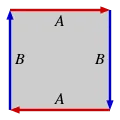
\includegraphics[scale=1]{images.png}
            \end{center}
            \caption{Modelo del espacio proyectivo $\bbm{R}P^2$ como cociente a partir de la identificación de los lados de un cuadrado.}
        \end{figure}

        es mapeado bajo $(i_2)_*$, así que:
        \begin{equation*}
            R=\left\{b^2\Big|[\gamma]\in\pi_1(U\cap V,x_0) \right\}
        \end{equation*}
        es tal que su cerradura normal visto como subgrupo de $\bbm{Z}$ es:
        \begin{equation*}
            \gen{\gen{R}}\cong 2\bbm{Z}
        \end{equation*}
        (pues $b$ es un generador de $\bbm{Z}$). Así que:
        \begin{equation*}
            \pi_1(\bbm{R}P^2,x_0)\cong\bbm{Z}/2\bbm{Z}
        \end{equation*}

        Para la botella de Klein...
    \end{sol}

    \begin{excer}
        Sea $X$ el subespacio de $\bbm{R}^2$ que consiste en la unión de los círculos $C_n$ de radio $n$ y centro $(n,0)$ para $n\in\mathbb{N}$. Calcula $\pi_1(x)$.
    \end{excer}

    \begin{sol}
        Para cada $n\in\mathbb{N}$ definamos:
        \begin{equation*}
            U_n=\left(\bigcup_{\substack{m\in\mathbb{N} \\ m\neq n}}C_n\right)
        \end{equation*}
    \end{sol}

    \begin{excer}
        Obtener el grupo fundamental del toro con Seifert-Van Kampen.
    \end{excer}

    \begin{sol}
        Considere el toro $\bbm{T}=\bbm{S}^1\times\bbm{S}^1$. Sean $x,y\in\bbm{T}$ puntos opuestos del toro. Tomemos $U=\bbm{T}\setminus\left\{p \right\}$ y $V=\bbm{T}\setminus\left\{q\right\}$. El conjunto $U\cap V=\bbm{T}\setminus\left\{p,q \right\}$ es arco-conexo y, además, se tiene que para $x_0\in U\cap V$:
        \begin{equation*}
            \pi_1(U,x_0)\cong\pi_1(V,x_0)\cong\gen{a,b|}
        \end{equation*}
        En efecto, lo probaremos para $\pi_1(U,x_0)$ (para el otro conjunto el proceso es análogo). Lo que estamos haciendo es \textit{ponchar} al toro y con ello, podemos retraer todos los puntos al conjunto $\bbm{S}^1\lor\bbm{S}^1$ como se muestra en la figura:

        \begin{minipage}{\textwidth}
            \begin{center}
                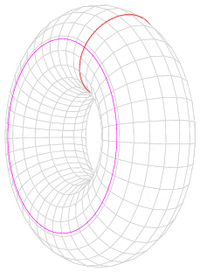
\includegraphics[scale=0.5]{torus.png}\\
                Figura \thefigcount. Toro $\bbm{T}$.
                \stepcounter{figcount}
            \end{center}
        \end{minipage}
        
        tal conjunto tiene como grupo fundamental a $\bbm{Z}*\bbm{Z}$. Por el Teorema de Van-Kampen se tiene que:
        \begin{equation*}
            \pi_1(\bbm{T},x_0)\cong(\bbm{Z}*\bbm{Z})*_{\pi_1(U\cap V,x_0)}\bbm{Z}*\bbm{Z}
        \end{equation*}
        obtengamos a $\pi_1(U\cap V,x_0)$. Se tiene que este espacio se retrae a $\bbm{S}^1\lor\bbm{S}^1\lor\bbm{S}^1$, que tiene como grupo fundamental a $\bbm{Z}*\bbm{Z}*\bbm{Z}$, por lo cual:
        \begin{equation*}
            \pi_1(\bbm{T},x_0)\cong F_2*_{F_3}F_2=\gen{a,b,c,d|R}
        \end{equation*}
        siendo $a$ y $c$ los círculos horizontales (en $U$) y, $b$ y $d$ los verticales (en $V$).

        Tomemos una clase de camino $[\gamma]$ en $\pi_1(U\cap V,x_0)$. Este camino se expresa como producto de $x,y,z$ de elementos en $F_3$ (en ese orden son los anillitos, siendo $y$ el horizontal). Se tiene que:
        \begin{itemize}
            \item $x$ y $z$ son mandados en $\pi_1(U,x_0)$ a $a$ y $a^{-1}$ (respectivamente), y $y$ a $b$.
            \item $x$ y $z$ son mandados en $\pi_1(U,x_0)$ a $c^{-1}$ y $c$ (respectivamente), y $y$ a $d$.
        \end{itemize}
        por lo que, la expresión de $[\gamma]$ es enviada a algo en $\gen{x,y,z}$ y luego a ese mismo producto cambiando algunas letras. En particular, se tiene que:
        \begin{equation*}
            c^{-1}a,d^{-1}b,\in R,
        \end{equation*}
        por lo que el producto amalgamado solo tiene dos elementos generadores. Más aún, se tiene que:
        \begin{equation*}
            xy\mapsto ab\quad\textup{y}\quad xy\mapsto c^{-1}d
        \end{equation*}
        por lo cual,
        \begin{equation*}
            d^{-1}cab \in R
        \end{equation*}
        por ende, las relaciones son:
        \begin{equation*}
            \begin{split}
                \pi_1(\bbm{T},x_0)&\cong\gen{a,b,c,d|a=c,d=c,b^{-1}a^2b=1}\\
                &\cong\gen{a,b|ab=a^{-1}b}\\
            \end{split} 
        \end{equation*}
        %Chance hay algo mal

        Era más simple con la identificación del toro como espacio cociente.
    \end{sol}

    \begin{excer}
        Sea $X$ el subespacio de $\bbm{R}^3$
    \end{excer}

    \section{Espacios Cubrientes}

    \begin{excer}
        Para un espacio cubriente $\cf{p}{\widetilde{X}}{X}$ y un subespacio $A\subseteq X$, sea $\widetilde{A}=p^{-1}(A)$. Muestre que la restricción $\cf{p|_{\widetilde{A}}}{\widetilde{A}}{A}$ es un espacio cubriente.
    \end{excer}

    \begin{proof}
        Sea $q=p|_{\widetilde{A}}$. Esta función es continua por ser la restricción de una funcioń continua, además es suprayectiva pues $f$ lo es.
        
        Veamos que cumple la condición deseada. Sea $x\in A$,en particular, $x\in X$, por lo que existe un abierto $U_x\subseteq X$ que contiene a $x$ tal que
        \begin{equation*}
            p^{-1}(U_x)=\bigsqcup_{\alpha\in I}V_\alpha
        \end{equation*}
        con $V_\alpha\cong U_x$ para todo $\alpha\in I$. Tomemos $V_x=U_x\cap A$. Este conjunto es abierto en $A$ tal que $x\in V_x$. Se cumple que:
        \begin{equation*}
            \begin{split}
                p^{-1}(V_x)&=p^{-1}(U_x\cap A)\\
                &=p^{-1}(U_x)\cap p^{-1}(A)\\
                &=\left(\bigsqcup_{\alpha\in I}V_\alpha\right)\cap\widetilde{A}\\
                &=\bigsqcup_{\alpha\in I}V_\alpha\cap\widetilde{A}\\
                &=\bigsqcup_{\alpha\in I}W_\alpha\\
            \end{split}
        \end{equation*}
        donde $W_\alpha=V_\alpha\cap\widetilde{A}$. Claramente la unión es disjunta pues originalmente era la unión disjunta de conjuntos. Veamos pues que la función $\cf{p\Big|_{W_\alpha}=q\Big|_{W_\alpha}}{W_\alpha}{V_x}$ es homeomorfismo. En efecto, sea $\alpha$. Como $p\Big|_{V_\alpha}$ es homeomorfismo entre $V_\alpha$ y $U_x$, se tiene que en particular que la función $\cf{q\Big|_{W_\alpha}}{W_\alpha}{q\Big|_{W_\alpha}(W_\alpha)}$ también lo es, donde el conjunto el conjunto:
        \begin{equation*}
            W_\alpha=V_\alpha\cap\widetilde{A}
        \end{equation*}
        es homeomorfo a:
        \begin{equation*}
            \begin{split}
                q\Big|_{W_\alpha}(W_\alpha)&=p\Big|_{V_\alpha}(W_\alpha)\\
                &=p\Big|_{V_\alpha}(V_\alpha\cap\widetilde{A})\\
                &=p\Big|_{V_\alpha}(V_\alpha)\cap p\Big|_{V_\alpha}(\widetilde{A})\\
                &=U_x\cap A\\
                &=W_x\\
            \end{split}
        \end{equation*}
        Se sigue pues que $\cf{q}{\widetilde{A}}{A}$ es espacio cubriente.
    \end{proof}

    \begin{excer}
        Sean $\cf{p_1}{\widetilde{X}_1}{X_1}$ y $\cf{p_2}{\widetilde{X}_2}{X_2}$ proyecciones cubrientes. Demuestre que la función $\cf{p_1\times p_2}{\widetilde{X}_1\times\widetilde{X}_2}{X_1\times X_2}$ también es una función cubriente.
    \end{excer}

    \begin{proof}
        Sea $q=p_1\times p_2$ dada por:
        \begin{equation*}
            q(\widetilde{x}_1,\widetilde{x}_2)=(p_1(\widetilde{x}_1),p_2(\widetilde{x}_2))
        \end{equation*}
        Claramente esta función es continua pues sus componentes son continuas, además es suprayectiva ya que también ambas funciones componentes son suprayectivas.
        
        Sea $x=(x_1,x_2)\in X_1\times X_2$, entonces existen $U_{ x_1}\subseteq X_1$ y $U_{ x_2}\subseteq X_2$ abiertos que contienen a $x_1$ y $x_2$ (respectivamente), tales que:
        \begin{equation*}
            p_1^{-1}(U_{ x_1})=\bigsqcup_{\alpha_1}V_{\alpha_1}\quad\textup{y}\quad p_2^{-1}(U_{ x_2})=\bigsqcup_{\alpha_2}V_{\alpha_2}
        \end{equation*}
        Tomemos $U_{x}=U_{x_1}\times U_{x_2}$. Este conjunto es abierto en $X_1\times X_2$ (con la topología producto o de caja). Se tiene que:
        \begin{equation*}
            \begin{split}
                p^{-1}(U_x)&=\left\{y\in\widetilde{X}_1\times\widetilde{X}_2\Big|p(y)\in U_{x_1}\times U_{x_1} \right\}\\
                &=\left\{(\widetilde{y}_1,\widetilde{y}_2)\in\widetilde{X}_1\times\widetilde{X}_2\Big|p(\widetilde{y}_1,\widetilde{y}_2)\in U_{x_1}\times U_{x_2} \right\}\\
                &=\left\{(\widetilde{y}_1,\widetilde{y}_2)\in\widetilde{X}_1\times\widetilde{X}_2\Big|p_1(\widetilde{y}_1)\in U_{x_1}\textup{ y }p_2(\widetilde{y}_2)\in U_{x_2} \right\}\\
                &=\left\{(\widetilde{y}_1,\widetilde{y}_2)\in\widetilde{X}_1\times\widetilde{X}_2\Big|\widetilde{y}_1\in p_1^{-1}(U_{x_1})\textup{ y }\widetilde{y}_2\in p_2^{-1}(U_{x_2}) \right\}\\
                &=p_1^{-1}(U_{x_1})\times p_2^{-1}(U_{x_2})\\
                &=\bigsqcup_{\alpha_1,\alpha_2}V_{\alpha_1}\times V_{\alpha_2}\\
                &=\bigsqcup_{\alpha}V_\alpha
            \end{split}
        \end{equation*}
        donde $V_\alpha=V_{\alpha_1}\times V_{\alpha_2}$ siendo $\alpha=(\alpha_1,\alpha_2)$ un indexador de esta familia. Veamos que la función $p\Big|_{V_\alpha}$ es un homeomorfismo entre $V_\alpha$ y $U_x$, para todo $\alpha$. En efecto, se tiene que las funciones:
        \begin{equation*}
            \cf{p\Big|_{ V_{\alpha_1}}}{V_{\alpha_1}}{U_{ x_1}}\quad\textup{y}\quad \cf{p\Big|_{ V_{\alpha_2}}}{V_{\alpha_2}}{U_{ x_2}}
        \end{equation*}
        son homeomorfismos, en particular al tenerse que $p\Big|_{V_\alpha}=p\Big|_{ V_{\alpha_1}}\times p\Big|_{ V_{\alpha_2}}$, entonces $p\Big|_{V_\alpha}$ es función continua, biyectiva, con biyección también continua. Así que $p\Big|_{V_\alpha}$ es homeomorfismo.

        Por tanto, $p=p_1\times p_2$ es función cubriente.
    \end{proof}

    \begin{excer}
        Sea $\cf{p}{\widetilde{X}}{X}$ un espacio cubriente con $X$ conexo. Si $p^{-1}(x_0)$ tiene $k$-elementos para algún $x_0\in X$, entonces $p^{-1}(x)$ tiene $k$-elementos para todo $x\in X$.
    \end{excer}

    \begin{proof}
        Supongamos que existe $x\in X$ tal que $p^{-1}(x)$ posee una cantidad distinta de $k$-elementos. Se tienen dos casos:
        \begin{itemize}
            \item $\abs{p^{-1}(x)}<k=\abs{p^{-1}(x_0)}$: 
        \end{itemize}
    \end{proof}

    \newcommand{\Hom}[1]{\ensuremath{\textup{Hom}\left(#1\right)}}

    \begin{mydef}
        Sea $X$ espacio topológico y $G$ un grupo. Una acción $G\curvearrowright X$ es una \textbf{acción de grupo continua} tal que el mapeo:
        \begin{equation*}
            g\cdot x\mapsto x
        \end{equation*}
        es continuo, para todo $g\in G$. En otras palabras, la acción es un homomorfismo entre el grupo $G$ y el grupo de todos los homeomorfismos de $X$ en $X$. En tal caso, se dice que $X$ es un \textbf{$G$-espacio}.
    \end{mydef}

    \begin{excer}
        Sea $X$ un $G$-espacio, es decir, $X$ es un espacio topológico en el que $G$ actúa. ¿Qué condiciones debemos pedir a la acción para que la función cociente $\cf{p}{X}{X/G}$ sea un espacio cubriente?
    \end{excer}

    \begin{sol}
        Como $X$ es un $G$-espacio, existe una acción de $G$ en $X$, es decir, un homomorfismo $\cf{\varphi}{G}{\Hom{X}}$ (donde el conjunto $\Hom{X}$ es el conjunto de homeomorfismos de $X$ en $X$).

        Se tiene que la función cociente:
        \begin{equation*}
            \cf{p}{X}{X/G},x\mapsto [x]_G
        \end{equation*}
        donde: $[x]_G=\left\{y\in X\Big|\exists g\in G\textup{ tal que }y=gx \right\}=G\cdot x$. Esta función es continua y suprayectiva, por lo que hay que ver cuándo se cumple la condición de los abiertos.

        Sea $x\in X$, debemos encontrar un subconjunto $U_{[x]_G}$ de $X/G$ tal que:
        \begin{equation*}
            p^{-1}(U_{[x]_G})=\bigsqcup_{\alpha}V_\alpha
        \end{equation*}
        siendo $V_\alpha$ conjuntos abiertos en $X$ y tales que $\cf{p\big|_{ V_\alpha}}{V_\alpha}{U_{[x]_G}}$ es un homeomorfismo para todo $\alpha$.
    \end{sol}

    \begin{propo}
        Sea $X$ un espacio conexo y localmente arco-conexo, entonces $X$ es arco-conexo.
    \end{propo}

    \begin{obs}
        No todo espacio arco-conexo es localmente arco-conexo.
    \end{obs}

    \begin{excer}
        Sean $\widetilde{X}$ y $\widetilde{Y}$ espacios cubrientes simplemente conexos de espacios arco-conexos y localmente arco-conexos. Muestre que si $X$ tiene el mismo tipo de homotopía que $Y$, entonces $\widetilde{X}$ tiene el mismo tipo de homotopía que $\widetilde{Y}$.
    \end{excer}

    \begin{proof}
        Sean $x_0\in X$ y tomemos $y_0=f(x_0)$. Por el teorema de clasificación de espacios de recubrimiento, existe una biyección entre los cubrientes de $X$ y $Y$, con los subgrupos de $\pi_1(X,x_0)$ y $\pi_1(Y,y_0)$. Al ser $X\simeq Y$, se tiene que la función:
        \begin{equation*}
            \begin{split}
                \cf{f_*}{\pi_1(X,x_0)}{\pi_1(Y,y_0)},\quad f_*([\gamma])\mapsto[f\circ\gamma]
            \end{split}
        \end{equation*}
        es un isomorfismo de grupos. En particular, se tienen los siguientes subgrupos de $\pi_1(X,x_0)$ y $\pi_1(Y,y_0)$:
        \begin{equation*}
            \pi_1(\widetilde{X},\widetilde{x}_0)\quad\textup{y}\quad\pi_1(\widetilde{Y},\widetilde{y}_0)
        \end{equation*}
        donde $\widetilde{x}_0\in\widetilde{X}$ y $\widetilde{y}_0\in\widetilde{Y}$ son tales que $x_0=p(\widetilde{x_0})$ y $y_0=q(\widetilde{y}_0)$ (con $\cf{p}{\widetilde{X}}{X}$ y $\cf{q}{\widetilde{Y}}{Y}$ los respectivos cubrientes).
        Por tanto, como ambos son el grupo trivial (pues son simplemente conexos) el isomorfismo $\cf{f_*}{\pi_1(X,x_0)}{\pi_1(Y,y_0)}$ debe ser tal que:
        \begin{equation*}
            f_*(\pi_1(\widetilde{X},\widetilde{x}_0))=\pi_1(\widetilde{Y},\widetilde{y}_0)
        \end{equation*}

        \begin{obs}
            Como $\widetilde{X}$ y $\widetilde{Y}$ son simplemente conexos, entonces tienen el mismo tipo de homotopía que un punto, esto es que $\widetilde{X}\simeq\left\{*\right\}$ y $\widetilde{Y}\simeq\left\{*\right\}$ por lo que, al ser $\simeq$ una relación de equivalencia, se sigue que $\widetilde{X}\simeq\widetilde{Y}$.
        \end{obs}
    \end{proof}

    \begin{excer}
        Encuentre todos los espacios conexos de 2 y 3 hojas de $\bbm{S}^1\lor\bbm{S}^1$ hasta homeomofismo.
    \end{excer}

    \begin{sol}
        
    \end{sol}

    \begin{excer}
        Construye el cubriente universal de los siguientes espacios: $\bbm{T}^n\times\bbm{R}P^2$ y $\bbm{S}^1\lor\bbm{S}^2$.
    \end{excer}

    \begin{sol}
        Veamos uno por uno:
        \begin{itemize}
            \item Para el espacio: $\bbm{T}^n\times\bbm{R}P^2$ basta con encontrar un cubriente universal de $\bbm{T}^n$ y otro de $\bbm{R}P^2$ tales que ambos sean simplemente conexos, luego por un ejercicio anterior se seguiría que el producto de ambos es cubriente univeral del producto de estos dos espacios y, como:
            \begin{equation*}
                \pi_1(X\times Y,(x_0,y_0))\cong\pi_1(X,x_0)\times\pi_1(Y,y_0)
            \end{equation*}
            entonces el producto de éstos dos cubrientes universales seguirá siendo cubriente universal.

            Recordemos que:
            \begin{equation*}
                \bbm{T}^n\cong\underset{n-\textup{veces}}{\underbrace{\bbm{S}^1\times\cdots\times\bbm{S}^1}}
            \end{equation*}
            por lo que, como $\bbm{S}^1$ tiene como un cubriente universal a $\bbm{R}$, se sigue que $\bbm{R}^n$ es cubriente universal de $\bbm{T}^n$.

            Ahora para $\bbm{R}P^2$, afirmamos que $\bbm{S}^2$ es cubriente universal de la esfera. En efecto, para ello recordemos que el espacio proyectivo es construído a partir de la identificación:
            \begin{equation*}
                \bbm{R}P^2=\bbm{S}^2/(x\sim-x)
            \end{equation*}
            Consideremos el mapeo cociente $\cf{q}{\bbm{S}^2}{\bbm{R}P^2}$ dado por:
            \begin{equation*}
                x\mapsto[x]=\left\{x,-x\right\}
            \end{equation*}
            esta función es continua y suprayectiva. Sea $[x]$ una clase y considere el abierto:
            \begin{equation*}
                U_{[x]}=q(U_x)\subseteq \bbm{R}P^2 
            \end{equation*}
            (ya que $q$ es función abierta) donde $U_x\subseteq\bbm{S}^2$ es tal que $x\in U_x$ y:
            \begin{equation*}
                U_x=B(x,\delta)\cap\bbm{S}^2
            \end{equation*} 
            donde $B(x,\delta)$ es una bola en $\bbm{R}^3$ de radio $d>0$ que es menor al radio de la esfera $\bbm{S}^2$. Se tiene que:
            \begin{equation*}
                q^{-1}(U_{[x]})
            \end{equation*}
            tiene dos componentes, dadas por:
            \begin{equation*}
                q^{-1}(U_{[x]})=U_x\sqcup U_{ -x}
            \end{equation*}
            y, $q\Big|_{U_x}$ es homeomorfismo (pues es en ese abierto continua, biyectiva y con inversa continua). Así que $\bbm{S}^2$ es cubriente universal de $\bbm{R}P^2$.

            Por tanto, $\bbm{R}^n\times\bbm{S}^2$ es cubriente universal de $\bbm{T}^n\times\bbm{R}P^2$.

            \item Para el espacio: $\bbm{S}^1\lor\bbm{S}^2$, veamos que el espacio:
            \begin{equation*}
                X=\bbm{R}\sqcup\left(\bigsqcup_{ m\in\bbm{Z}}\bbm{S}^2  \right)/\left\{m\sim p_m,\forall m\in\bbm{Z}\subseteq\bbm{R} \right\}
            \end{equation*}
            donde $p_m$ es el polo norte de la $m$-ésima 2-esfera en la unión disjunta es cubriente universal. En efecto, no se complicado verificar (usando Van-Kampen) que este espacio es simplemente conexo. sea $\cf{p}{X}{\bbm{S}^1\lor\bbm{S}^2}$ dada por:
            \begin{equation*}
                p(s)=\left\{
                    \begin{array}{lcr}
                        e^{ 2\pi is} & \textup{ si } & s\in\bbm{R} \\
                        \pi(s) & \textup{ si } & s\in X\setminus\bbm{R}\\
                    \end{array}
                \right.
            \end{equation*}
            donde $\cf{\pi}{\bigsqcup_{ m\in\bbm{Z}}\bbm{S}^2}{\bbm{S}^2}$ es la proyección de un elemento de cualquier 2-esfera en la otra 2-esfera, la cual es una función cubriente. Claramente esta función es suprayectiva y continua (por el lema del pegado y por ser $s\mapsto e^{2\pi is}$ $\pi$ funciones continuas). Veamos que cumple la condición de los abiertos. Se tienen tres casos:
            \begin{itemize}
                \item $x\in\bbm{R}\setminus\bbm{Z}$, entonces existe un entero $m\in\mathbb{Z}$ tal que $m<x<m+1$. Tomando este intervalo se sigue, al ser $s\mapsto e^{ 2\pi is}$ cubriente universal de $\bbm{S}^1$, que tomando el abierto correspondiente en ese cubrente se sigue el resultado.
                \item $x\in X\setminus\bbm{R}$, existe un abierto $U_x$ en $\bbm{S}^2$ tal que $x\in U_x\subseteq\bbm{S}^1\setminus\left\{1\right\}$. De forma inmediata se sigue que $p^{-1}(U_x)$ cumple la condición deseada.
                \item Si $x\in\mathbb{Z}$, entonces tomando los dos abiertos resultantes de las dos funciones cubrientes y haciendo su unión, se tiene el resultado.
            \end{itemize}
            por los tres incisos se sigue el resultado.
        \end{itemize}
    \end{sol}

    \begin{excer}
        Sean $\cf{p}{\widetilde{X}}{X}$ y $\cf{q}{\widetilde{Y}}{Y}$ dos cubrientes universales. Muestre que para cada función $\cf{f}{X}{Y}$ existe una función $\cf{\widetilde{f}}{\widetilde{X}}{\widetilde{Y}}$ tal que:
        \begin{equation*}
            f\circ p=q\circ\widetilde{f}
        \end{equation*}
    \end{excer}

    \begin{proof}
        
    \end{proof}

    \begin{excer}
        Demuestra la siguiente proposición: Si $\cf{p}{(E,e_0)}{(X,x_0)}$ y $\cf{p'}{(E',e_0')}{(X,x_0)}$ son ambos espacios cubrientes simplemente conexos de $X$, entonces existe un único homeomorfismo $\cf{\varphi}{(E',e_0')}{(E,e_0)}$ tal que $p\circ\varphi=p'$.
    \end{excer}

    \begin{proof}
        
    \end{proof}

    \begin{excer}
        Para cualquier $n>0$, sea $C_n$ el círculo con centro $\left(\frac{1}{n},0\right)$ y radio $\frac{1}{n}$, defina $X=\bigcup_{ n=1}^\infty C_n$. Muestre que este espacio no tiene cubriente universal.
    \end{excer}

\end{document}